\documentclass[aspectratio=169]{beamer}

\usepackage[utf8]{inputenc}
\mode<presentation>
{
  \usetheme{Darmstadt}      % or try Darmstadt, Madrid, Warsaw, ...
  \usecolortheme{beaver} % or try albatross, beaver, crane, ...
  \usefonttheme{serif}  % or try serif, structurebold, ...
  \setbeamertemplate{navigation symbols}{}
  \setbeamertemplate{caption}[numbered]
  \setbeamertemplate{footline}[frame number]
  \setbeamertemplate{headline}{}
} 
\usepackage{graphicx}
\usepackage[english]{babel}
\usepackage[utf8]{inputenc}
\usepackage[T1]{fontenc}
\usepackage{bm}
\usepackage{amssymb}
\usepackage{amsmath}
\usepackage{physics}
\usepackage{bm}
\usepackage{leftidx}
\usepackage{mathtools}
\usepackage{tikz}
\usepackage{gensymb}
\usepackage{listings}
\usepackage{svg}
\pdfsuppresswarningpagegroup=1

\begin{document}
\AtBeginSection[]{
  \begin{frame}
  \vfill
  \centering
  \begin{beamercolorbox}[sep=8pt,center,shadow=true,rounded=true]{title}
    \usebeamerfont{title}\insertsectionhead\par%
  \end{beamercolorbox}
  \vfill
  \end{frame}
}

\title[Your Short Title]{Control of a Hurricane Hunting Aircraft}
\author{Corey Spohn, Jacob Pelster, Rachel Oliver, and Zvonimir Stojanovski}
\institute{MAE 6780 Multivariable Control Theory}
\date{\today}

\begin{frame}
  \titlepage
\end{frame}

\begin{frame}{Aircraft Dynamics}
    \begin{itemize}
        \item State
        \begin{equation*}
            \mathbf{x} = \begin{bmatrix}
                \mathbf{v}_B^T &
                \mathbf{r}_I^T &
                \boldsymbol{\omega}_B^T &
                \boldsymbol{\Theta}^T
            \end{bmatrix}^T
        \end{equation*}
        \item $I$ is the inertial frame; $B$ is the body frame
        \item Kinematics
        \begin{equation*}
            \dot{\mathbf{r}}_I = \mathbf{H}_B^I \mathbf{v}_I \qquad
            \dot{\boldsymbol{\Theta}} = \mathbf{L}_B^E \boldsymbol{\omega}_B
        \end{equation*}
        \item Overall dynamics
        \begin{equation*}
            \dot{\mathbf{x}} = \mathbf{f}(\mathbf{x},\mathbf{u},t)
        \end{equation*}
    \end{itemize}
\end{frame}

\begin{frame}{Hurricane Model}
A hurricane's wind field can be written as a radial velocity, $V_r$, that varies by radius, $r$, from hurricane center to plant, example below taken from Kalourazi 2020.
    \begin{columns}
    \begin{column}{0.55\textwidth}
        \begin{align}
        V_r = 
        \begin{cases}
                V_{max} \left( {\frac{r}{R_{max}}\right)^{\frac{3}{2}}, & r <
                R_{max} \\
                V_{max} \left( \frac{2 R_{max} r}{r^2 + R_{max}^2} \right), & r \geq R_{max} 
        \end{cases}
        \end{align}
        \end{column}
        \begin{column}{0.45\textwidth}
            \begin{figure}
            \centering
            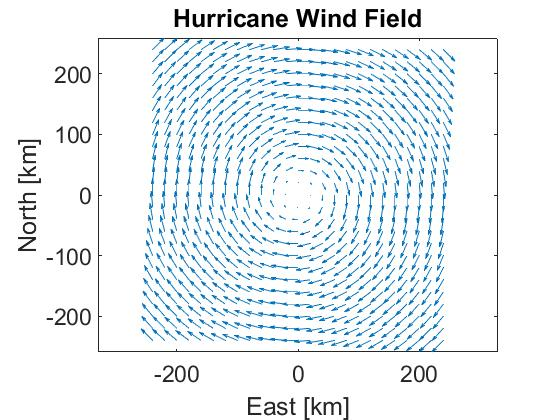
\includegraphics[width=1\textwidth]{HurricaneWindField.jpg}
        \end{figure}
        \end{column}
    \end{columns}
\end{frame}

\begin{frame}[t]
    \frametitle{Model Predictive Control (MPC) Intuition}
    %\framesubtitle{subtitle}
    Model predictive control is a fairly broad field of controls, all of which have the following characteristics
    \begin{itemize}
        \item Using a model to predict future outputs
        \item Calculating control inputs using the predicted future outputs and a cost function
        \item Applying the first step of the control input calculated, observing the true output at
            the step, moving the time horizon forward one step, and repeating
    \end{itemize}
    \begin{figure}
        \centering
        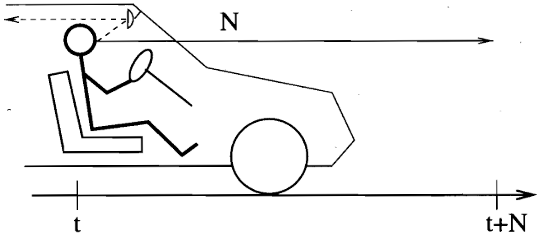
\includegraphics[scale=0.4]{MPC_analogy.png}
        \caption{MPC analogy, Camacho and Bordons 1999}
        \label{fig:my_label}
    \end{figure}
\end{frame}

\begin{frame}{MPC pros/cons}
    \begin{columns}
    
    \begin{column}{0.5\textwidth}
    \centering
    Pros\\
    \hrule
    \hfill
    \begin{itemize}
        \item Works well with MIMO systems
        \item Can be applied to many different kinds of systems, including unstable systems
        \item Control inputs can be defined with various control laws
        \item Performs exceptionally when future outputs are known
        \item Can handle constraints on both the control inputs and model outputs
    \end{itemize}
    \end{column}
    \begin{column}{0.5\textwidth}
    \centering
    Cons\\
    \hrule
    \hfill
    \begin{itemize}
        \item MPC is an online process that requires a processor with enough computing power and memory to handle the optimization in real time
        \item It is non-trivial to choose appropriate weights for terminal and control costs with a complex MIMO system
        \item It is non-trivial to choose the prediction horizon, control horizon, and time-step
    \end{itemize}
    \end{column}
    \end{columns}
\end{frame}

\begin{frame}{Our MPC Process}
    \begin{itemize}
        \item Create discrete time linear plant, disturbance, and noise models
        \item Estimate future plant outputs, $y$, based on the current state, $x_c$
        \item Calculate the next control input by solving the quadratic programming optimization
            problem with the plant outputs, constraints, and a cost function.
        \item Apply the control step
        \item Calculate the next $x_c$
        %\item Incremental control implementation\\
            %$ \mathbf{u}(t\rightarrow{t+1}) = -\mathbf{K}_{mpc}*\mathbf{x}(t)$
    \end{itemize}
    \begin{figure}
        \centering
        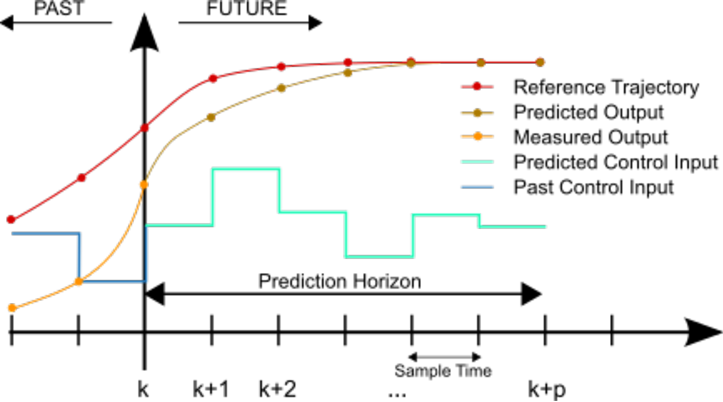
\includegraphics[width=0.5\textwidth]{MPC_scheme_basic.pdf}
        \caption{MPC Strategy, from Wikipedia}
    \end{figure}
\end{frame}

\begin{frame}[t]
    \frametitle{Estimation}
    %\framesubtitle{}
    We create a state vector $x_{c}$ and a prediction horizon $p$
    \begin{align*}
        x_c^{T}(k) = 
\begin{bmatrix}
    x_p^{T}(k) & x^{T}_{id}(k) & x^{T}_{od}(k) & x^{T}_{n}(k) \\
\end{bmatrix}
    .\end{align*}
    \begin{itemize}
        \item $x_p$ is the plant model state vector
        \item $x_{id}$ is the input disturbance model state vector
        \item $x_{od}$ is the output disturbance model state vector
        \item $x_{n}$ is the measurement noise model state vector
    \end{itemize}
    Then estimate the future states at steps $i=1, 2, \ldots, p$, denoted $x_c\left( k+i|k \right)$, using a Kalman filter,
    which are then used to predict the predicted plant outputs 
    \begin{align*}
        y\left( k+i|k \right) = C x_c\left( k+i|k \right) 
    .\end{align*}
\end{frame}

\begin{frame}[t]
    \frametitle{Solving the Optimization Problem}
    %\framesubtitle{subtitle}
    The quadratic program (QP) optimization problem consists of
    \begin{itemize}
        \item Decision ($z_k$), a vector of future control inputs
        \item The cost function
            \begin{align*}
                J(z_k) = J_y(z_k) + J_u (z_k) + J_{\Delta u}(z_k) + J_{\epsilon} (z_k)
            .\end{align*}
            \begin{itemize}
                \item $J_y$ is the cost of keeping outputs near their reference tracking values
                \item $J_u$ is cost of keeping manipulated variables near their target values
                \item $J_{\Delta u}$ constrains the how fast manipulated variables can be adjusted
                \item $J_{\epsilon}$ is the cost of constraint violations
            \end{itemize}
    \end{itemize}
    For $J_y$, $J_u$, and $J_{\Delta u}$ we create scale factors, $s$, and tuning weights, $w$, that
    multiply the difference between the target/reference value $r$ and the current value $y$, and sum for
    all state variables $n_y$ for the duration of the prediction horizon $p$
    \begin{align*}
        J_{y, u, \Delta u}(z_k) = \sum_{j=1}^{n_y} \sum_{i=1}^{p} \left\{ \frac{w_{i, j}}{s_j}
        \left[ r_j \left( k+i|k \right) - y\left( k+i|k \right)  \right]  \right\} 
    .\end{align*}
\end{frame}

\begin{frame}[t]
    \frametitle{Solving the Optimization Problem}
    %\framesubtitle{subtitle}
    For $J_{\epsilon}$ we define a constraint violation penalty weight $\rho_{\epsilon}$ and a
    variable that represents the worst case constraint violation at the current step $\epsilon_k$ 
    \begin{align*}
        J_{\epsilon}(z_k) = \rho_{\epsilon} \epsilon_k ^2
    .\end{align*}
    Currently we're finding our optimal decision $z(k)$ with the default MATLAB QP
    solver which implements an active-set solver based on the KWIK algorithm. The first element of
    the decision is $u(k)$ which we can implement.
    %Then we solve the optimization problem based on the general form QP problem
    %\begin{align*}
        %\min_{z_k}\left( \frac{1}{2}z_k^{T} H z_k \right) 
    %.\end{align*}
    %$H$ here is the Hessian matrix based off of the cost function
\end{frame}

%\begin{frame}[t]
    %\frametitle{Estimation}
    %%\framesubtitle{subtitle}
    %A Kalman filter is used to predict future states
    
%\end{frame}

\begin{frame}[t]
    \frametitle{MPC in MATLAB}
    %\framesubtitle{subtitle}
    \begin{itemize}
        \item Matlab includes a model predictive control toolbox
        \item Requires a discrete-time, state-space system plant
        \item The MPC object includes:
        \begin{itemize}
            \item Hard and soft constraints to the manipulated and observed variables
            \item Weights for quadratic cost function
            \item Scale factors account for orders of magnitude difference between variables in the cost function
            \item Disturbances are implemented into the MPC object in varying ways depending on type. Input/Output and Known/Unknown
            \item The provided "review" command helps assess the stability and computational feasibility of the described MPC object
        \end{itemize}
        \item Once balanced, the MPC controller can be simulated with the "mpcmove" or "sim" command
    \end{itemize}
\end{frame}



\begin{frame}{Model Predictive Control Results}
    \begin{columns}
        \begin{column}{0.55\textwidth}
            \begin{figure}
                \centering
                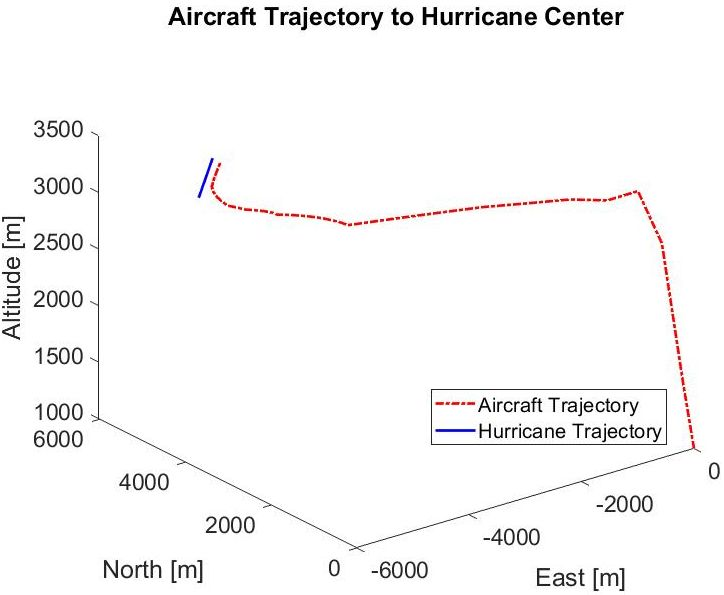
\includegraphics[width=1\textwidth]{MPC_Disturbance_3D.jpg}
            \end{figure}
        \end{column}
        \begin{column}{0.45\textwidth}
            \begin{figure}
                \centering
                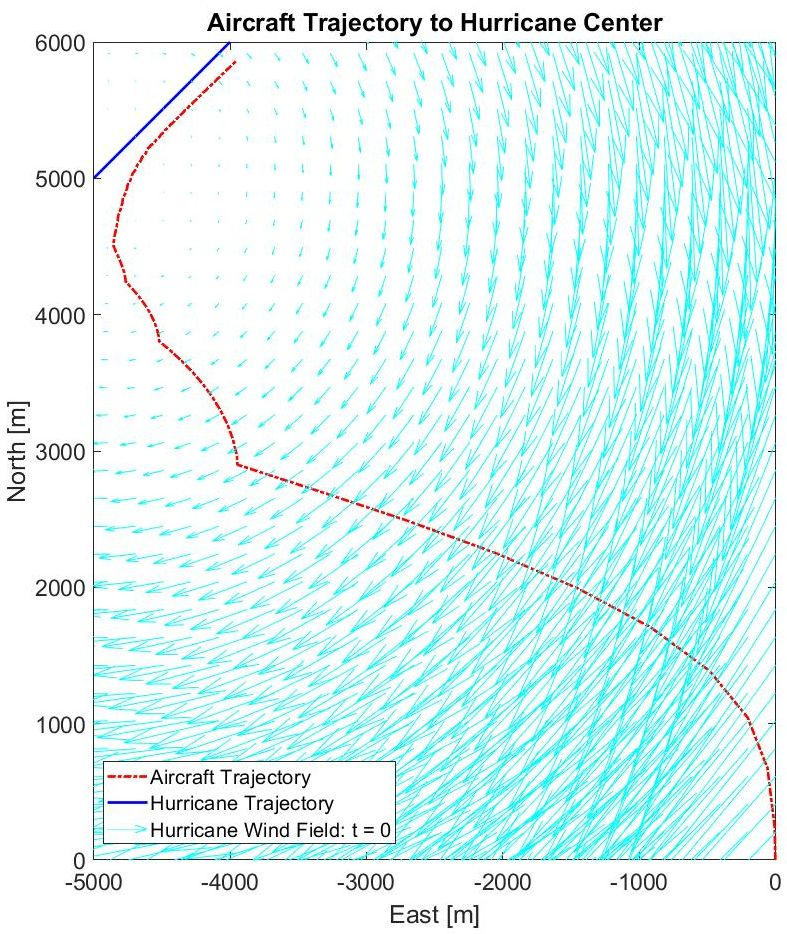
\includegraphics[width=1\textwidth]{MPC_Disturbance_2D.jpg}
            \end{figure}
        \end{column}
    \end{columns}
\end{frame}

\begin{frame}{Model Predictive Control Results}
    \begin{columns}
        \begin{column}{0.5\textwidth}
            \begin{figure}
                \centering
                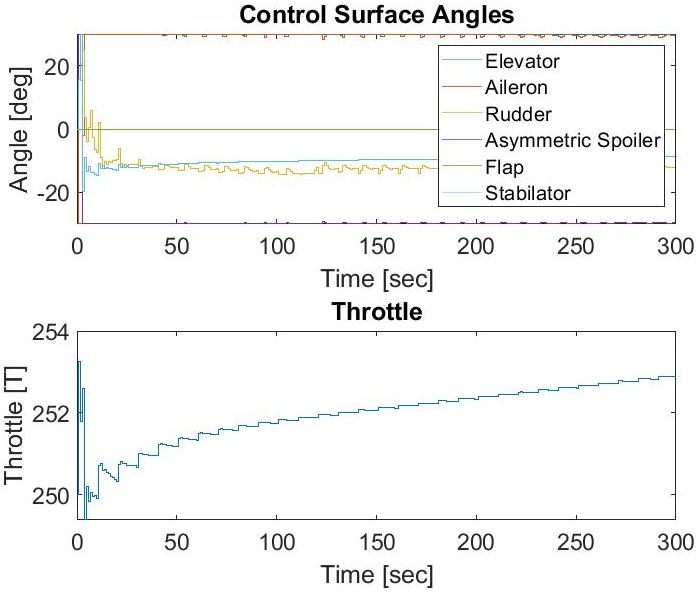
\includegraphics[width=1\textwidth]{MPC_Disturbance_Controls.jpg}
            \end{figure}
        \end{column}
        \begin{column}{0.5\textwidth} 
            \begin{figure}
                \centering
                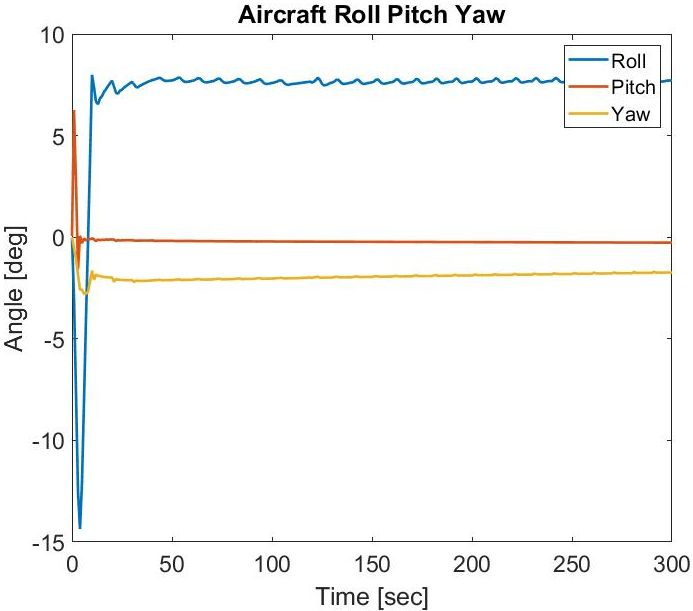
\includegraphics[width=1\textwidth]{MPC_Disturbance_Roll_Pitch_Yaw.jpg}
            \end{figure}
        \end{column}
    \end{columns}
\end{frame}

\begin{frame}[t]
    \frametitle{Sliding Mode Control Motivation: Phase Space Constraint}
    %\framesubtitle{test}
    %Sliding Mode Control

        Suppose we have a single variable system with $x_2=\dot{x}_1$ where the following is true: $$x_2+Cx_1=0$$ With phase portrait:
        \begin{figure}[htbp]
        \centering
        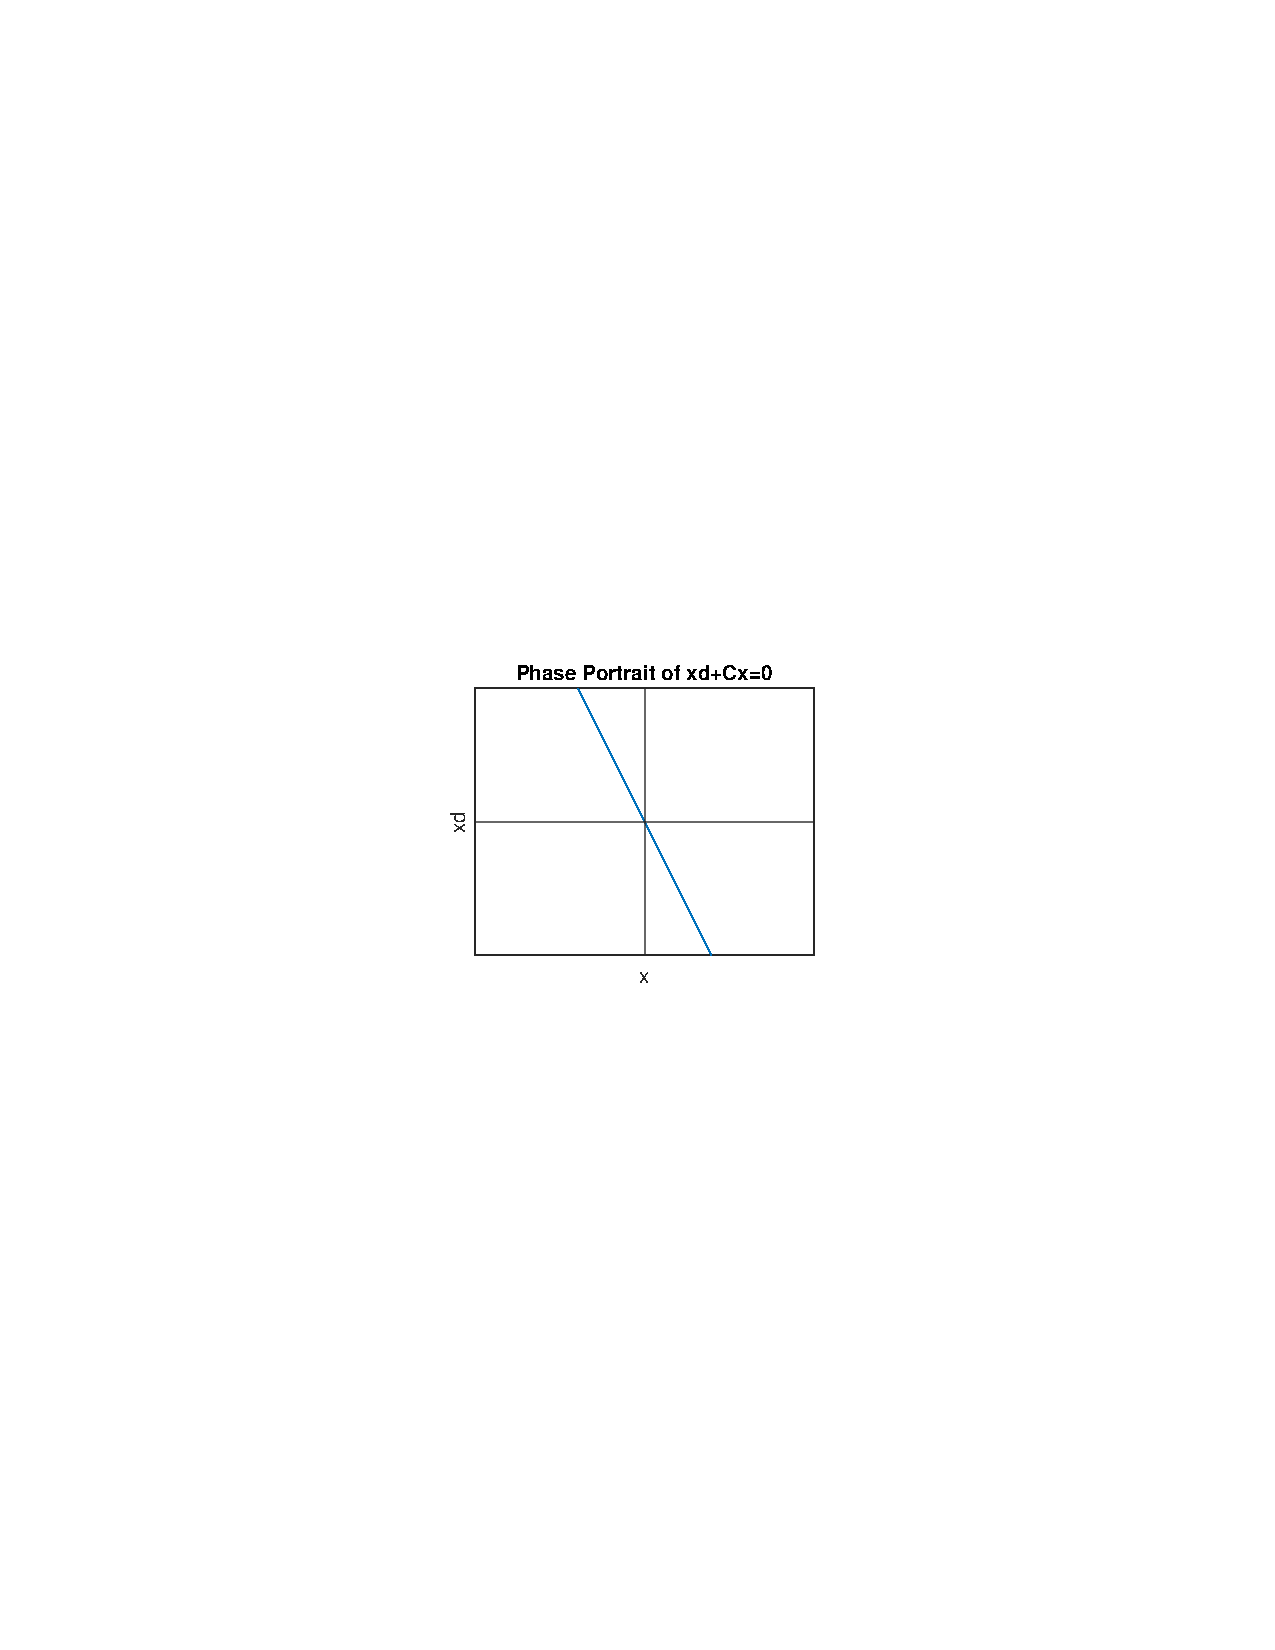
\includegraphics[trim=4.5cm 11.2cm 3cm 11cm,clip, width=0.5\textwidth]{Phase portrait.pdf}
    \end{figure}
    
    The solution is a first order system and has a solution of the form: $$x_1=x_1(t_0)e^{-Ct}$$ Which converges to zero if C>0.
\end{frame}
\begin{frame}
    \frametitle{Sliding Mode Control Motivation: Desired Behavior}
    
    Consider the second order system:
    \begin{align*}
    \dot{X}&=
    \begin{bmatrix}
    \dot{x_1}\\
    \dot{x_2}
    \end{bmatrix}\\
    &=
    \begin{bmatrix}
    x_2\\
    f_2(X,t)+g_2(X,u,t)
    \end{bmatrix}
    \end{align*}
    \begin{itemize}
    \item It would be desirable if the dynamics obeyed $0=x_2+Cx_1$ from above.
    \item Define $\sigma=x_2+Cx_1$.
    
    \item If $\sigma=0$, the dynamics of the system meet the desired and the system converges.
    \item If $\sigma\neq0$ we would want $\sigma\to0$
    This can be ensured by $\sigma\dot{\sigma}<0$.
    \begin{itemize}
    \item If $\sigma>0$ then $\dot{\sigma}$ must be negative and $\sigma$ is decreasing (approaching 0 from above).
    \item If $\sigma<0$ then $\dot{\sigma}$ must be positive and $\sigma$ is increasing (approaching 0 from below).
    \end{itemize}

    \end{itemize}
\end{frame}
\begin{frame}
    \frametitle{Sliding Mode Control Motivation: Meeting the requirements}
    We have two requirements:
    \begin{itemize}
        \item $\dot{\sigma}$ fits with the required dynamics of the system.
        \item $\dot{\sigma}$ has the opposite sign of $\sigma$.
    \end{itemize}
    
    The first requirement implies:
    \begin{itemize}
        \item $\dot{\sigma}=\dot{x_2}+C\dot{x_1}=f_2(X,t)+g_2(X,u,t)+Cx_2$
    \end{itemize}
    
    If the first requirement is met then we can design a $\dot{\sigma}$ that meets the second requirement, one such is:
    \begin{itemize}
        \item $\dot{\sigma}=-\eta sign(\sigma)$
    \end{itemize}
    Which is not the only option. 
    
    We use the sign function to ensure that the state reaches $\sigma=0$ in finite time.
    
    Setting them equal:
    \begin{itemize}
        \item $f_2(X,t)+g_2(X,u,t)+Cx_2=-\eta sign(\sigma)$
    \end{itemize}
    
    
\end{frame}
\begin{frame}
    \frametitle{Sliding Mode Control Motivation: The Result}
    If we can find a u such that the above equation is satisfied, then the state approaches $\sigma=0$ when $\sigma\ne0$ and obeys the dynamics $0=x_2+Cx_1$ when $\sigma=0$.
    \begin{figure}[htbp]
        \centering
        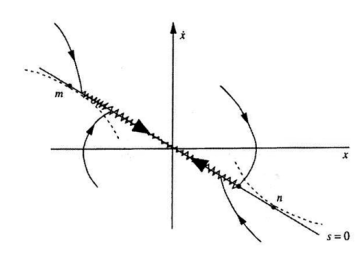
\includegraphics[width=0.5\textwidth]{Sliding Mode Figure.png}
        \caption{Sliding Mode Control Example, Utkin 2008 \cite{UtkinSMC}}
    \end{figure}
    

\end{frame}
\begin{frame}
    \frametitle{Sliding Mode Control Motivation: Chatter}
    \begin{itemize}
        \item In most cases u is function of $sign(\sigma)$
        \item $sign(\sigma)$ is discontinuous.
        \item If the actuators cannot switch infinitely, there will be deviation from the required control.
        \item The control when $\sigma>0$ will overshoot into $\sigma<0$ and conversely.
    \end{itemize}
    \begin{figure}[htbp]
        \centering
        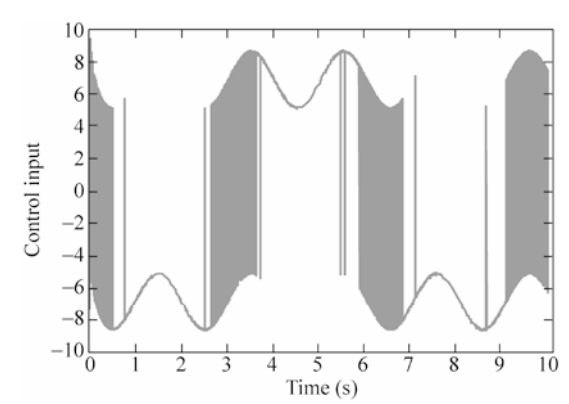
\includegraphics[width=0.3\textwidth]{Sliding Mode Chatter.png}
        \caption{Infinitely Fast Response in Control with Sign(), Liu and Wang, 2011 \cite{LiupingWang2009}}
    \end{figure}
    This can be alleviated partially by using the sigmoid function.
\end{frame}
\begin{frame}{Sliding Surface for Aircraft Control}
    \begin{itemize}
        \item We want the aircraft to follow a specified state $\mathbf{r}^*_I(t)$, $\boldsymbol{\Theta}^*(t)$
        \item Define the state errors
        \begin{equation*}
            \Delta \mathbf{r}_I = \mathbf{r}_I - \mathbf{r}_I^* \qquad \Delta \boldsymbol{\Theta} = \boldsymbol{\Theta}-\boldsymbol{\Theta}^*
        \end{equation*}
        \item We want to confine the aircraft's motion to the hypersurface on which
        \begin{equation*}
            \Delta \dot{\mathbf{r}}_I= -K_r \delta \mathbf{r}_I \qquad \Delta \dot{\boldsymbol{\Theta}} = -K_\theta \delta \boldsymbol{\Theta}
        \end{equation*}
        \item Combined with kinematics, this defines our ``sliding surface''
        \begin{equation*}
            \boldsymbol{\sigma}(\mathbf{x}) = 
            \begin{bmatrix}
                \mathbf{H}_B^I \mathbf{v}_I - \dot{\mathbf{r}}_I^* + K_r ( \mathbf{r}_I - \mathbf{r}_I^*) \\
                \mathbf{L}_B^E \boldsymbol{\omega}_B - \dot{\boldsymbol{\Theta}}^* + K_\theta(\boldsymbol{\Theta}-\boldsymbol{\Theta}^*) 
            \end{bmatrix} = \mathbf{0}
        \end{equation*}
        \item Aircraft state is exponentially stable on sliding surface
    \end{itemize}
\end{frame}

\begin{frame}{Sliding Surface for Aircraft Control}
    \begin{itemize}
        \item Sliding surface can be expressed as
        \begin{equation*}
            \boldsymbol{\sigma} = \mathbf{S}\mathbf{x} - \mathbf{S}^*\mathbf{x}^* = \mathbf{0}
        \end{equation*}
        where
        \begin{equation*}
            \mathbf{S}(\mathbf{x}) = \begin{bmatrix}
                \mathbf{H}_B^I & K_r\mathbf{I} & \mathbf{0} & \mathbf{0} \\
                \mathbf{0} & \mathbf{0} & \mathbf{L}_B^E & K_\theta\mathbf{I}
            \end{bmatrix}
        \end{equation*}
        \item Then
        \begin{equation*}
            \dot{\boldsymbol{\sigma}} = \dot{\mathbf{S}}\mathbf{x} + \mathbf{S}\dot{\mathbf{x}} - \dot{\mathbf{S}}^*\mathbf{x}^* - \mathbf{S}\dot{\mathbf{x}}^*
        \end{equation*}
    \end{itemize}
\end{frame}

\begin{frame}{Aircraft Sliding Mode Control}
    \begin{itemize}
        \item Linearize dynamics with respect to controls $\mathbf{u}$
        \begin{equation*}
            \dot{\mathbf{x}} = \mathbf{f}(\mathbf{x},\mathbf{u},t) = \mathbf{h}(\mathbf{x},\mathbf{u},t) + \mathbf{B} (\mathbf{u} - \mathbf{u}^*)
        \end{equation*}
        \item Substitute into sliding mode derivative
        \begin{equation*}
            \dot{\boldsymbol{\sigma}} = \dot{\mathbf{S}}\mathbf{x} + \mathbf{S}[\mathbf{h}(\mathbf{x},\mathbf{u},t) + \mathbf{B} (\mathbf{u} - \mathbf{u}^*)] - \dot{\mathbf{S}}^*\mathbf{x}^* - \mathbf{S}\dot{\mathbf{x}}^*
        \end{equation*}
    \end{itemize}
\end{frame}

\begin{frame}{Aircraft Sliding Mode Control}
    \begin{itemize}
      \item Choose a constant $L$ such that
        \begin{equation*}
            |\{\dot{\mathbf{S}}\mathbf{x} - \mathbf{S}\mathbf{h}(\mathbf{x},\mathbf{u},t) - \dot{\mathbf{S}}^*\mathbf{x}^* - \mathbf{S}\dot{\mathbf{x}}^*\}_i| < L
        \end{equation*}
        \item If we set $\mathbf{S}\mathbf{B} (\mathbf{u} - \mathbf{u}^*) = -L \mathrm{sgn}(\boldsymbol{\sigma})$, we can prove that
        \begin{equation*}
            \frac{d}{dt}\left(\frac{1}{2}\boldsymbol{\sigma}^T\boldsymbol{\sigma}\right) = \boldsymbol{\sigma}^T\dot{\boldsymbol{\sigma}} < 0
        \end{equation*}
        so the system reaches $\boldsymbol{\sigma}=\mathbf{0}$ in finite time
    \item Finally, we obtain the control
    \begin{equation*}
        \mathbf{u} = \mathbf{u}^* -L (\mathbf{S}\mathbf{B})^{-1} \mathrm{sgn}(\boldsymbol{\sigma})
    \end{equation*}
        \item In practice, use sigmoid instead of sgn to avoid ``chatter''
        \end{itemize}
\end{frame}


\begin{frame}{Sliding Mode Control Results}
    \centering
    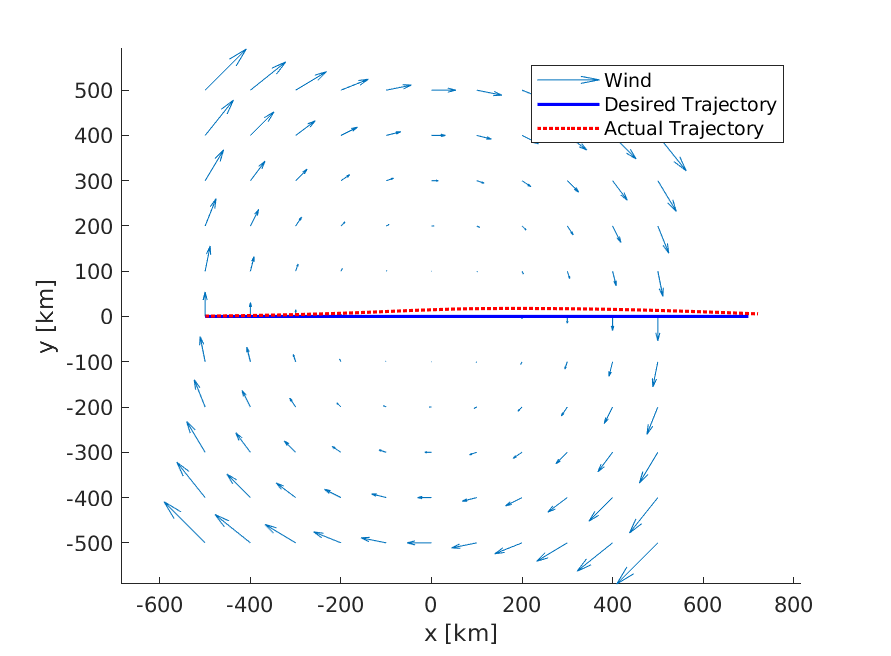
\includegraphics[width=0.49\textwidth]{sm_hurricane.png} 
    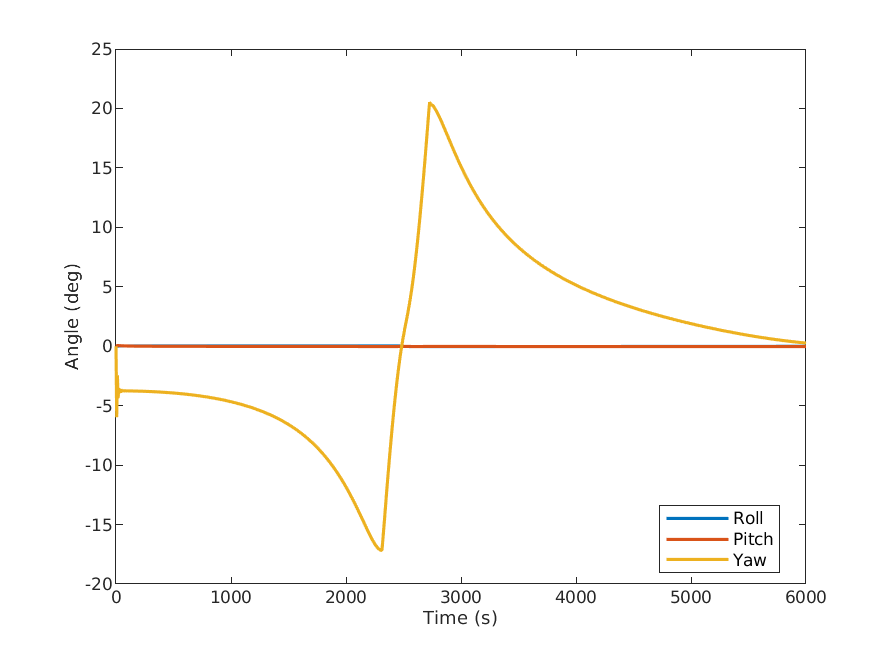
\includegraphics[width=0.49\textwidth]{sm_rpy.png}
\end{frame}

\begin{frame}{Way Ahead - Combining MPC and Sliding Mode}
    Discrete Sliding Mode:
    \begin{itemize}
        \item $\sigma(k)=Cx(k)$
        \item New reaching condition $|\sigma(k+1)|-|\sigma(k)|<0$ (The next iteration is always less in magnitude.)
    \end{itemize}
    Reaching Law:
    \begin{align*}
        \begin{cases}
           s_r(k+p)=(1-qT)s_r(k+p-1)\xi(k)\\
            -\epsilon Tsgn(s(k+p-1))\psi(k)\\
            s_r(k)=s(k)
        \end{cases}
    \end{align*}
    
    
    Where $\xi$ is a factor to allow for an exponential reaching law outside of the vicinity of the sliding mode and $\psi$ acts as a smoother to reduce chatter in the vicinity of the sliding mode.
    
    (1-qT) is related to the time delay.
    
    $\epsilon$ is how forceful the reaching law is.\break
    \break
    Nizar 2013 \cite{NizarMPCSMC}; Xiao et. al., 2006 \cite{XiaoMPCSMC}
\end{frame}
\begin{frame}{Way Ahead - Combining MPC and Sliding Mode}
    We can predict the future sliding function $s_p$ (function, not mode) at every time until the horizon.
    \break
    
    Want to optimize the predicted sliding function to minimize the difference between it and the reference sliding mode trajectory, as well as minimize the control.\break
    
    Cost function (k is current step):
    $$j_p=\sum\limits_{j=1}^{N}[s_p(k+j)-s_r(k+j)]^2+\sum\limits_{l=0}^{M-1}g[u(k+l)]^2$$
    Where g is a weight.\break
    Can optimize this to solve for u, to find the optimal u!\break (note: $s_p(n)$ is a function of u(k),...,u(n)) \break
    \break
    Nizar 2013 \cite{NizarMPCSMC}; Xiao et. al., 2006 \cite{XiaoMPCSMC}
\end{frame}

\begin{frame}{References}
    \nocite{*}
    \footnotesize
    \bibliographystyle{ieeetr}
    \bibliography{references}
\end{frame}
\end{document}



\begin{frame}
    \frametitle{Sliding Mode Control Motivation: Creating the Constraint}
    Given that, if a system fits the requirement $x_2+Cx_1=0$ it would be desirable to make this true. If we define the variable s as: $s=x_2+Cx_1$, then when s=0, the requirement is met. So our goal is to make s converge to 0, in order to make the constraint true. To do this, we note that, if $s\dot{s}<0$ then s will always decrease if positive or always increase if negative.(If $s\dot{s}<0$, then if s>0, then $\dot{s}$ must be less than zero, so s will decrease. If s<0, then $\dot{s}$ must be greater than zero, so s will increase.) To ensure that this is the case, we would like $\dot{s}$ to always have the opposite sign as s, so we pick $\dot{s}=-k sign(s)$. This isn't $\dot{s}$, but what we would like $\dot{s}$ to be. We additionally have that $\dot{s}$, as required by the dynamics, is: $\dot{s}=\dot{x_2}+C\dot{x_1}$, where:
    \[
    \dot{X}=
    \begin{bmatrix}
    \dot{x_1}\\
    \dot{x_2}
    \end{bmatrix}
    =f(X,t)+g(X,u,t)
    \]
    Which is dependent on the free variable u, so we are free to control $\dot{s}$ as the wanted constraint if we can solve for u. Noting, this we set our desired $\dot{s}$ to the $\dot{s}$ required by the dynamics, dependent on our control.
    $$\dot{s}=f_2(X,t)+g_2(X,u,t)+Cf_1(X,t)+Cg_1(X,u,t)=-k sign(s)$$, and if we can solve for u, then: $u=h(X,t)-k sign(s)$
\end{frame}

\begin{frame}
    \frametitle{Sliding Mode Control Motivation: Simplifying}
    If we assume that our system is linear time invariant, then the dynamics are described by:
    \[
    \begin{bmatrix}
    \dot{x_1}\\
    \dot{x_2}
    \end{bmatrix}
    =
    \begin{bmatrix}
    A_{11} & A_{12}\\
    A_{21} & A_{22}\\
    \end{bmatrix}
    \begin{bmatrix}
    x_1\\
    x_2
    \end{bmatrix}
    +
    \begin{bmatrix}
    B_1\\
    B_2
    \end{bmatrix}
    u
    \]
    Meaning we can solve the above equation for the control:
    $$(B_1+B_2)u=-CA_{11}x_1-CA_{12}x_2-A_{21}x_1-A_{22}x_2-k sign(s)$$
    Then, if u satisfies the above equation, the desired constraint $\dot{s}=\dot{x_2}+C\dot{x_1}$ is met, and the system.
\end{frame}
\begin{frame}[t]
    \frametitle{Sliding Mode Control}
    %\framesubtitle{test}
    %Sliding Mode Control
    \begin{itemize}
        \item Want to confine state $\mathbf{x}$ to surface $\boldsymbol{\sigma}(\mathbf{x})=\mathbf{0}$ (``sliding surface'') on which system is stable
        \item Control proportional to $\mathrm{sgn}(\boldsymbol{\sigma})$ brings state to sliding surface in finite time (but often better to use sigmoid function to avoid ``chatter'')
        \item Stability conditions depend only on bounds of system dynamics
        \item Can be combined with Model Predictive Control
    \end{itemize}
\end{frame}
